\section{The Decision Required From Eight PMUs}
\label{sec:narrative-problem}

At every report, the task is to decide whether the recent trajectory contains a physical intervention and, if so, identify its family, source and onset. Detection is the existence decision; classification chooses the physical operator; localization chooses a bus or branch. Those outputs need not become reliable at the same time. We keep the estimated physical onset $\widehat\tau$ separate from the time at which an alarm or diagnosis is emitted.

The network has 39 buses, but the prescribed PMU set is
\begin{equation}
 \mathcal P=\{2,5,6,10,19,22,29,39\}.
 \label{eq:narrative-pmus}
\end{equation}
Voltage is measured at each PMU bus. Current is measured at a specified branch terminal, which can differ from that bus. The causal implementation uses 47 coordinates: eight voltage magnitudes, eight voltage angles, eight current magnitudes, seven current angles, eight absolute frequencies and eight ROCOFs, at 30 reports/s. BUS39 current angle is excluded because its interpretation remains partially validated. The BUS5 current terminal retains the provisional historical 5--6 assignment. These are declared measurement assumptions, not identities inferred from classification accuracy.

\begin{figure*}[t]\centering
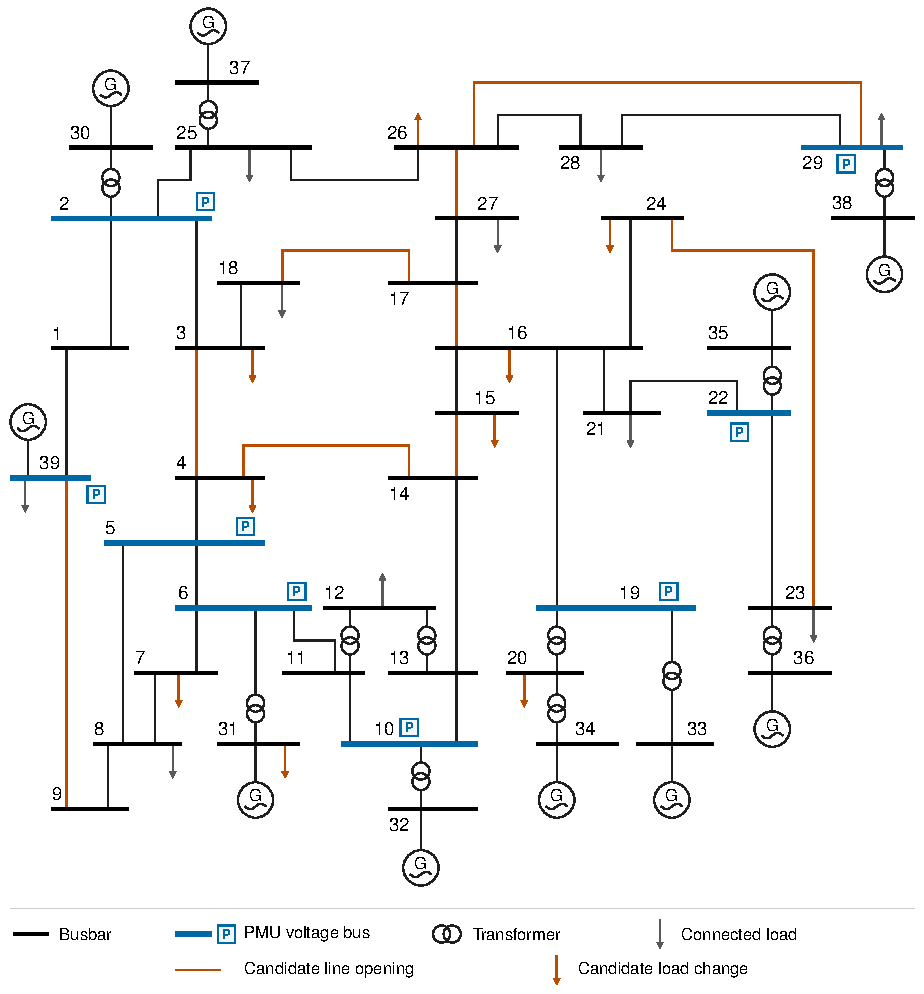
\includegraphics[width=.92\textwidth]{figures/generated/narrative_topology.pdf}
\caption{What is measured and what is hypothesized. The frozen causal bank contains nine load buses and nine line assets within the 39-bus network; eight blue buses carry PMUs. An unmeasured candidate is inferred through its network response at those PMUs. Orange branches are candidate interventions, not current-sensor assignments. Coordinates are schematic and do not define electrical distance.}
\label{fig:narrative-topology}\end{figure*}

The physical model is
\begin{align}
 \dot x&=f_q(x,z,u;\theta),&0&=g_q(x,z,u;\theta),\label{eq:narrative-dae}\\
 y_k&=\mathcal M_q(x_k,z_k;\theta_M)+b+\varepsilon_k.\label{eq:narrative-measurement}
\end{align}
Here $x$ contains machine and control dynamics, $z$ the algebraic network variables, $q$ the topology/intervention mode, and $\theta_M$ the measurement convention. The measurement map includes gains, phase references, orientation and the causal frequency/ROCOF estimator. A machine's rotor speed is not substituted for bus frequency.

An intervention hypothesis is $h=(e,c,\tau,a,d)$: family, source, onset, severity and duration. A load changes its local P/Q setpoints. A line opening switches its branch primitive; it is not approximated as a load change. For the supported impulse-free switches,
\begin{equation}
 x(\tau^+)=x(\tau^-),\qquad g_{q^+}(x(\tau^-),z(\tau^+),u;\theta)=0.
 \label{eq:narrative-switch}
\end{equation}
The algebraic voltage/current response may jump even though dynamic states remain continuous. Physical restoration reverses the intervention operator. It does not return the machines to their pre-event state, so electrical recovery can continue after OFF.

\begin{table}[t]\centering\small
\caption{Scope of the executed causal component. The source is an intervention asset; it is not necessarily a measured PMU bus.}\label{tab:narrative-scope}
\begin{tabularx}{\columnwidth}{@{}lXX@{}}\toprule
Case & Physical operator & Executed claim\\\midrule
Normal & No intervention & Monitor after startup\\
Load & Local P/Q factor; optional restoration & Nine candidate buses\\
Line & Branch open; optional reclose & Nine candidate branches\\
Fault/generation & Different shunt/input/trip operators & Outside this causal test\\
Missing/bad data & Measurement-integrity mechanism & Outside C01\\
Unknown & Unresolved diagnosis & Not a new physical family\\\bottomrule
\end{tabularx}\end{table}

The generator stores event schedules and true states separately from the PMU stream. Inference receives the nominal network, permitted calibration and reports through the current time. It receives no source, switch time, true R/X realization or solver state. Initial operating context and noise scale are estimated from 300 startup reports; monitoring begins after the inherited 12-s warmup. The startup contract assumes no intervention in that prefix.
